\subsection{Dns Script}
\begin{figure}[htp]
\centering
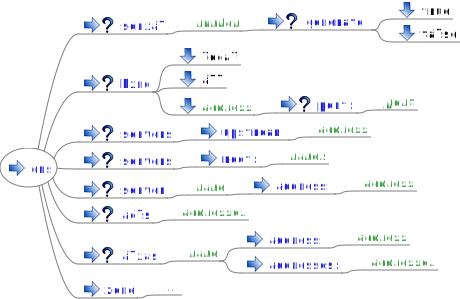
\includegraphics[angle=90,height=0.99\textheight]{dns_service_script}
\label{fig:dns_script_statements}
\caption{Dns Script Statements}
\end{figure}


\TheStatement{dns}
\TheStatement*[dns]{dns \{ serial bind\_address zone \}}

Entry point in the dns script.

\TheStatement[dns:serial]{serial}
\TheStatement*[dns!serial]{serial \Arg{number} [, generate: true|false]}

Sets the serial \Arg{number} of the zone records.
The serial number can be any number, it is added to the automatically
generated serial. The DNS service needs the serial number to be updated
for all records that have been changed. The service can create serial
numbers based on the current date but the user needs to update this
serial number if the records are changed more then once in a day.
If generate is set to \code{true} then the serial number is added to
the automatically generated serial, otherwise the serial number is used 
as specified.

\TheStatement[serial:bind_address]{bind\_address}
\TheStatement*[dns!bind\_address]{bind\_address \Arg{address}}

The IP \Arg{address} or the host name on which the dns server should listen
to connections. Defaults to the localhost address \qcode{127.0.0.1}.

\TheStatement[dns:zone]{zone}
\TheStatement*[dns!zone]{zone \Arg{name}, \Arg{primary}, \Arg{email} [, \Arg{address}] [, \Arg{ttl}] [, \{ ttl refresh retry expire minimum\_ttl ns\_record a\_record mx\_record cname\_record \} ]}

Adds a new DNS zone. The \Arg{name}, the \Arg{primary} DNS server and 
the \Arg{email} address of the zone are required. An A-record for the zone
can be created if the IP \Arg{address} of the zone is specified. If the
\Arg{ttl} time is specified it is set for the A-record.

\TheStatement[dns:ttl]{ttl}
\TheStatement*[dns!ttl]{ttl \Arg{time}}

Sets the time to live \Arg{time}. The default time to live time is 24 hours.

\TheStatement[dns:refresh]{refresh}
\TheStatement*[dns!refresh]{refresh \Arg{time}}

Sets the refresh \Arg{time}. The default refresh time is 8 hours.

\TheStatement[dns:retry]{retry}
\TheStatement*[dns!retry]{retry \Arg{time}}

Sets the retry \Arg{time}. The default retry time is 2 hours.

\TheStatement[dns:expire]{expire}
\TheStatement*[dns!expire]{expire \Arg{time}}

Sets the expire \Arg{time}. The default expire time is 4 days.

\TheStatement[dns:minimum_ttl]{minimum\_ttl}
\TheStatement*[dns!minimum\_ttl]{minimum\_ttl \Arg{time}}

Sets the minimum time to live \Arg{time}. The default minimum time is 1 day.

\TheStatement[dns:ns_record]{ns\_record}
\TheStatement*[dns!ns\_record]{ns\_record \Arg{name} [, \Arg{address}] [, \{ ttl \}]}

Adds a new NS-record with the specified name. If the \Arg{address}
of the record is specified then a new A-record will be created that maps this 
name to the specified address.

\TheStatement[da:a_record]{a\_record}
\TheStatement*[da!a\_record]{a\_record \Arg{name} [, \Arg{address}] [, \{ ttl \}]}

Adds a new A-record with the specified \Arg{name} and \Arg{address}.

\TheStatement[dmx:mx_record]{mx\_record}
\TheStatement*[dmx!mx\_record]{mx\_record \Arg{name} [, \Arg{address}] [, \{ ttl priority \}]}

Adds a new MX-record with the specified name. If the \Arg{address}
of the record is specified then a new A-record will be created that maps this 
name to the specified address.

\TheStatement[dmx:priority]{priority}
\TheStatement*[dmx!priority]{priority \Arg{priority}}

Sets the priority for the MX-record. The default priority is 10.

\TheStatement[da:cname_record]{cname\_record}
\TheStatement*[da!cname\_record]{cname\_record \Arg{name} \Arg{alias} [, \{ ttl \}]}

Adds a new CNAME-record with the specified \Arg{name} and \Arg{alias}.
